\chapter*{Summary}
\chaptermark{}
\addcontentsline{toc}{chapter}{Summary - Samenvatting}

{\Large\bf
  The Weak Phase \phis and Penguin Topologies.
}
\vspace*{0.05\textwidth}

Within the domain of modern pysics there exists a particular field of research
that attempts to answer a fundamental question about the natural world. This
question follows intuitivelly when observing the natural world and it troubled
philospphers since the ancient times. These philosophers attempted to understand
which are the fundamental blocks that build the world around them. Remarkably
enough after more that 2000 years since Democitus, who is commonly accepted as
the first person that introduced the idea of idivisible blocks of nature named
atoms (or \textgreek{άτομα} in Greek), contemprary scientists still have not found a definite
answer on the fundamental blocks of nature. So far, it seems that the observable
universe consists of a handful of elementary particles, which are clasified in two
distinct categories, namely {\it gauge bosons}, responsible for mediating all the
known fundamental forces of nature (with the exception of gravity) and {\it fermions}
which are the constituents of matter. There are 5 gauge bosons and 12 fermions.
Fermions can be divided further into {\it quarks}, which constitute composite
particles like the proton. A typical {\it lepton} is the electron which orbits
the nucleus of all atoms.

\subsubsection{Particle Physics and The Standard Model}
The state of the art mathematical framework necessary to describe the interactions between the
fermions is called the \textit{Standard Model} of Particle Physics \cite{sm-glashow,sm-weinberg,sm-salam}.
Describing an interaction in this context means being able to predict the probability for a certain
outcome in a (fundamental) particle colision. Given the fact that energy and mass can convert
from one to the other, the type of the initial and final particles is not the same. For example,
two initial quarks can colide, or more precicely annihilate, and produce an electron-positron pair.
This is counter intuitive compared to the clasical, non-quantum, description of particle collisions,
where the atomic structure of particles does not change. Thus, the established predictive power of
the Standard Model is an important achievement of particle physicists. Furthermore, the recently
discovered Higgs boson \cite{higgs-cms,higgs-atlas}, which plays a special role in explaining how
particles acquire mass, makes the Standard Model robust.

Despite the its sucess in describing the outcome of particle interactions, there are certain
established phenomena and observations that Standard Model does not account for.
Perhaps the most striking one is the absence of any description about the most familiar,
yet the weakest, force of nature, meaning gravity. Or perhaps the observed matter-antimatter
asymmetry in the universe \cite{more-cpv-huet,more-cpv-gavela_I,more-cpv-gavela_II}.
Note that antimatter is a well understood state of matter that has its quantum numbers sign,
such as electric charge, flipped with respect to matter. The above phenomena are a few
examples that reveal the incompletness of the model. Thus the scientific method compels
scientists to continue testing Standard Model predictions and look for ways to improve it.
Any significant diviation from these predictions could hint the presence of
{\it New Physics} beyond the established model.


\subsubsection{The \lhcb Detector}
In order to find new physics we do big big xperiments. The best one is ....
\begin{itemize}
\item \lhc cern most powerfull accelrator
\item \lhcb dedicated bfys experiment, unique capabilities, high signal purity. maybe mention proximity to beam and pid.
\item future increase of low pt muon efficiency extents NP reach.
\end{itemize}


\subsubsection{\CP Violation}
According to the dominant consensus regarding the matter-antimatter balance in the
universe, it is believed that during the big bang matter and antimatter existed at
equal proportions. This idea invites the notion of the so called Charge-Parity (\CP)
symmetry between matter and antimatter. Perfect \CP symmetry when it comes to particle
interactions imply that nature interacts both with matter and antimatter at the same rate.
However, at current time the observable universe seems to be almost entirely populated by
matter. Given this observation, the origin of this violation of the \CP symmetry follows
as a natural question.

The established idea that nature favours processes where the final particles are matter
and not antimatter particles is indeed captured by the Standard Model. It addition, it
is intreasting to point out that the origin of \CP violation is very closely releated
to the mechanism that the fermions aquire mass, which is the Higgs boson. However,
despite the fact that the Standard Model allows for the presence of \CP violation,
it cannot account for the observed ammount of matter-antimatter asymmetry.
Hence, other sources of \CP violation beyond the Standard Model have to be active.

The ammount of \CP violation is typically quantified by several parameters for which
the predicted by the Standard Model values have to be compared against the experimentally
measured values. Potential descrepancy between the prediction and the measured value
provide hints for the presence of New Physics. It is intreasting to point out that all these paramters have to yield
a consistent picture with each other. This offers a powerful discrimination between alternative models that might
modify Standard Model predictions. In other words these alternative models have to
modify all the \CP violating parameters in a consistent way.


\subsubsection{The Weak Phase \phis and the \BsJpsiKst decay}
Violation of the \CP symmetry in particle physics typicaly manifests itself when comparing
the rate, or probability, of two particle decays. The two decays are releated by a \CP symmetry.
In other words one decay consits of matter while the other of antimatter particles.
Given the established presence of \CP violation in nature the previous rates are not equal.

An intreasting particle decay to measure \CP violation and compare it with the Standard Model
predicion is the \BsJpsiPhi decay.
% This particular decay is appealing since the prediction for the amount of \CP
% violation is very precise. In addition, the \BsJpsiPhi decay has a high signal purity as well
% as a high detection efficiency, making it appealing from an experimental point of view.
Furthermore, the way \CP violation manifests itself in this parituclar decay is intriguing
as it involves the quantum mechanical interference of two decay amplitudes, see \equref{app_interf_amp}.
Note that the intereference is possible since both the \Bs particle and its antimatter counterpart,
\Bsb, can decay to the same final state $f$, as shown in \figref{app_interference}.

\begin{equation}
  \centering
A(\BsJpsiPhi) = |\color{red}{A1} + \color{blue}{A2}| = \color{red}{A1}^2 + \color{blue}{A2}^2 + A1*A2*\cos\delta
  \label{app_interf_amp}
\end{equation}


\begin{figure}[h]
  \centering
  \resizebox{0.4\textwidth}{!}{\begin{picture}(0,0)%
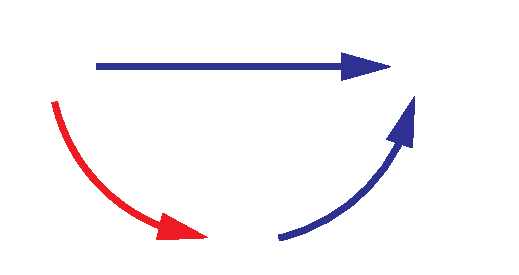
\includegraphics{Figures/Chapter1/decay_CMYK.pdf}%
\end{picture}%
\setlength{\unitlength}{4144sp}%
%
\begingroup\makeatletter\ifx\SetFigFont\undefined%
\gdef\SetFigFont#1#2#3#4#5{%
  \reset@font\fontsize{#1}{#2pt}%
  \fontfamily{#3}\fontseries{#4}\fontshape{#5}%
  \selectfont}%
\fi\endgroup%
\begin{picture}(3939,2094)(2644,-2188)
\put(3286,-736){\makebox(0,0)[rb]{\smash{{\SetFigFont{25}{30.0}{\sfdefault}{\mddefault}{\updefault}{\color[rgb]{0,0,0}$\Bs$}%
}}}}
\put(5761,-736){\makebox(0,0)[lb]{\smash{{\SetFigFont{25}{30.0}{\sfdefault}{\mddefault}{\updefault}{\color[rgb]{0,0,0}$\ffig$}%
}}}}
\put(4501,-421){\makebox(0,0)[b]{\smash{{\SetFigFont{25}{30.0}{\sfdefault}{\mddefault}{\updefault}{\color[rgb]{0,0,1}}%
}}}}
\put(5581,-1771){\makebox(0,0)[lb]{\smash{{\SetFigFont{25}{30.0}{\sfdefault}{\mddefault}{\updefault}{\color[rgb]{0,0,1}}%
}}}}
\put(3331,-1771){\makebox(0,0)[rb]{\smash{{\SetFigFont{25}{30.0}{\sfdefault}{\mddefault}{\updefault}{\color[rgb]{1,0,0}}%
}}}}
\put(4501,-2041){\makebox(0,0)[b]{\smash{{\SetFigFont{25}{30.0}{\sfdefault}{\mddefault}{\updefault}{\color[rgb]{0,0,0}$\Bsb$}%
}}}}
\end{picture}%
}
  \caption{The two interfering decay paths leading to the same final state.}
  \label{app_interference}
\end{figure}

The parameter quantifing \CP violation in the \BsJpsiPhi decay is the so called weak phase \phis.
The Standard Model prediction of the latter parameter as well as its most precice measurement by
\lhcb is:

\begin{subequations}
  \label{app_phis_lhcb_theo}
  \begin{align}
  \centering
  \phiS{\lhcb}           &=  -0.010 \pm 0.039(\text{total})  \;\; \text{rad},
  \label{app_phis_lhcb}\\
  \phiS{SM,tree}  &= -0.03761 {}^{+0.00073}_{-0.00082}  \;\; \text{rad}.
  \label{app_phis_theo}
\end{align}
\end{subequations}

\noindent The goal of measuring \phis is to look for New Physics effects that Standard Model
does not predict. Given the measuremnt of \equref{app_phis_lhcb} it follwos that \phis is comaptible
with the prediction and any New Physics effects that might apear in \phis must be small.
From an experimental point of view the situation is just now becoming intrasting
since the statistical uncertainty of the experimental measuremnt is approaching the Standard
Model prediction. Thus, with the upgraded \lhcb detector \phis enters a high precision era
of measurements, where along with other observables will most likely be able to point towards
a prticular New Physics model.

However, entering this promising high precision era comes along with an important consideration
that has to be taken into acount in order to make a robust claim about the presence of New Physics
in \phis. In particular there are certain subleading effects within the Standard Model, comming from
the so called {\it penguin topologies}, that the \phis measurement of \equref{app_phis_lhcb} does not
take into account, see \figref{}. These subleading effects shift the Standard Model prediction, $\phis^{\tiny \text{SM,tree}}$,
by a small amount, $\Delta\phiS{SM,peng}$. Considering also the fact that, as implied by \equref{app_phis_lhcb_theo},
potential New Physics in \phis are small: One understands that contributions to \phis from Standard
Model subleading penguin topologies are imposible to disentangle from potential New Physics contributions,
which also shift the Standard Model prediction by, $\Delta\phis^{\tiny \text{NP}}$.
The situation is deppicted in following equation:

\begin{equation}
\centering
 \phis^{\text {eff}} = \phis^{\tiny \text{SM,tree}} + \Delta\phiS{SM,peng} + \Delta\phis^{\tiny \text{NP}}.
 \label{app_phis_sm_peng}
\end{equation}

\noindent Note that increasing the precision of $\phis^{\text {eff}}$ does not help at all in distinguishing
between $\Delta\phiS{SM,peng}$ and $\Delta\phis^{\tiny \text{NP}}$. In addition, the subleading penguin
topologies are supressed with respect to tree in the \BsJpsiPhi decay by two orders of magnitude.
This suppresion factor is reflected to a large undertainty in the estimated penguin topology contributions,
$\Delta\phiS{SM,peng}$, if the \BsJpsiPhi decay channel is used. Thus once again it is not possible to
make a strong claim about New Physics contrubutions to \phis.

Given the above mentioned limitations it becomes mandatory to estimate contributions from
penguing topology to \phis using a different decay chanell, \eg the \BsJpsiKst decay as suggested by
\cite{}\cite{}. The latter is a decay that has identical tree and penguin topologies with \BsJpsiPhi,
with the only difference being one of the quarks forming the \Pphi particle, see \figref{app_jpsiphi_tree_peng}.
Note that the two decay diagrams, tree and penguin, in \BsJpsiKst are not suppressed with resect to eachother.
Thus the uncertainty to $\Delta\phiS{SM,peng}$ does not suffer from any supression when measured using the
\BsJpsiKst decay channel. On the other the presence of a \Kstarz particle instead of a \Pphi introduces
uncertainty to $\Delta\phiS{SM,peng}$, since the assumption of perfect symmetry between an \squark and \dquark quarks
needs to be made. In turns out that the loss in precision using the \BsJpsiKst decay channel does not
forbid a useful estimation of $\Delta\phiS{SM,peng}$ and it is thus indeed possible to get a handle on
potential New Physics contribution to $\Delta\phis^{\tiny \text{NP}}$.

{\color{red} Mention jpsi rho as well, }

\begin{figure}[t]
  \begin{subfigure}{0.5\textwidth}
    \raggedright
    {\scalebox{1}{\sffamily \input{Figures/Chapter1/tree}}}
    \label{app_jpsiphi_tree}
  \end{subfigure}%
  \hfill
  \begin{subfigure}{0.5\textwidth}
    \raggedleft
    {\scalebox{1}{\sffamily %%BoundingBox: -5 0 121 170
%%HiResBoundingBox: -5 0 120.57008 169.36447

\begin{fmffile}{Figures/Chapter1/penguin}
  \fmfframe(17,-25)(31,-25){
    \begin{fmfgraph*}(115,170)
      \fmfstraight
      \fmfleft{i0,i1,i2,i3,i4,i5}
      \fmfright{o0,o1,o2,o3,o4,o5}
      \fmf{fermion,tension=1.8,label.side=left,label=b}{v5,i3}
      \fmf{fermion,tension=1.5,right=0.2,label.side=left,label={\hspace*{18pt}u,,c,,t}}{v2,v5}
      \fmf{gluon,tension=2}{v4,v2}
      \fmf{dbl_dashes,tension=0}{v4,v2}
      \fmf{fermion,tension=0.3,right=0.2,label.side=left }{v3,v2}
      \fmf{boson,tension=0.6,left=0.3,label=W$^+$,label.side=left}{v3,v5}
      \fmf{fermion,label=c,tension=0.9,right=0.3,label.side=left}{o4,v4}
      \fmf{fermion,label=c,tension=0.9,right=0.3,label.side=left}{v4,o3}
      \fmf{fermion,label=s,label.side=left}{o2,v3}
      \fmffreeze
      \fmf{fermion,tension=0.7,label=s,label.side=left}{v1,o1}
      \fmf{fermion,tension=1,label.side=left,label=s}{i2,v1}
      %\fmf{phantom,tension=0.4}{v4,v1}
      \fmf{phantom,tension=0.4}{v3,v1,v5}
      \fmf{plain,right=0.2}{i2,i3}
      \fmf{plain,left=0.2,label=$\Bs$}{i2,i3}
      \fmf{plain,right=0.2,label=$\phi$}{o1,o2}
      \fmf{plain,left=0.2}{o1,o2}
      \fmf{plain,right=0.2,label=$\jpsi$}{o3,o4}
      \fmf{plain,left=0.2}{o3,o4}
    \end{fmfgraph*}
  }
\end{fmffile}
}}
    \label{app_jpsiphi_peng}
  \end{subfigure}
    \caption{Leading order {\it tree} (left) and subleading penguin (right) \BsJpsiPhi decay topologies.}
  \label{app_jpsiphi_tree_peng}
\end{figure}

\subsubsection{Analysing Particle Collisions}
Having introduced the penguin parameter $\Delta\phiS{SM,peng}$ it is intreasting to point out some
aspects releated to the experimental measurement itself and thus highlight the pipeline followed from
the recorded raw particle collisions and the final result.

To begin with the recorded \BsJpsiKst and \BsJpsiRho decays, necessary to extract the penguin paramter,
have to be processed such that the presence of background, noise, is suppressed as much as possible.
Background processes are in general introduced due to finite experimental resolution. Having a clean
sample is always desired; particularly in the case of the \BsJpsiKst decay which has a low probability
of occuring with respect to the \BdJpsiKst decay, see \figref{}. Furthermore, the spin configurations
in the \BsJpsiPhi decay , where \Jpsimumu and \phiKK, is such that the direction of the final state
particles, mumu and KK, becoems relevant and have to be accounted for by a multi dimensional model.

At that point it is usefull to emphasize the fact that in particle physics, parameters of intereset
require a sufficiently large number of recorded particle collisions, data, in order to be estimated.
This welcomes a statistical aproach to aprameter estiamtion where, the larger the data size is the
more precise the estimate on the paramter of intereset becomes. The same holds for a sample size that
is as free of background, noise, as possible. Furthermore, finite experimental resolution as well as
varius the detector responce could introduce biases and have to be taken into account by the previous
multi dimensional model.

Once the data have been cleaned from the presence of background and all the experimental effects are
properly taken into account the model, which depends on the paramter of itnereset, is fitted to the data.
The fitting process is based on the maximum likelihood paramter estimation.
How does fitting work.{\color{red} Maybe add a paragraph on the likelihood}
Explain that the likelihood is a product of probabilities. It is intuitive that you look for its maximum.
The likelihood gives back: What is the probability to observe the data given this paramter of intereset.
At its max it gives the best paramter of intereset given the data. Note that in fact you want the inverse
but thats another story..

\subsubsection{Result, Impact and Conclusion}

Having performed the likelihood fit of the multidimensional model to the data and following \cite{}Robert
the final result for the paramters of intereset are:

The shifts $\DeltaPhisJpsiPhi{k}$ quoted in \equref{delta_phis_result}
suggest that contributions of penguin topologies to the \BsJpsiPhi decay amplitude are
small, $<1^\circ$. Given the also small \phis measured value from \lhcb shown in \equref{phis_lhcb}
it becomes mandatory to control penguin contributions in future \phis measurements.
Furthermore, the sensitivity from the experimental side is interesting with respect to
the Standard Model prediction, see \equref{phis_lhcb_theo}. Thus, potential deviations from this
prediction is going to play a central role in future and more precise \phis measurements.
Increasing the amount of data in the \lhc \runtwo might not be enough to yield
a significant claim on the presence of physics beyond the Standard Model and hence
the upgraded \lhcb detector becomes important in the pursuit for New Physics with \phis in the future.
The result implies that the penguin contribution to the \phis is small, blah.
